%%%%%%%%%%%%%%%%%%%%%
%                                              %
%                 Experiment M-9               %
%                Harmonic Motion               %
%                                              %
%%%%%%%%%%%%%%%%%%%%%

%\labChapter{M}{Simple \& Damped Harmonic Motion}
\labChapter{M}{Simple \& Damped Harmonic Motion with Springs \& Glider on Level Air Track}
\label{lab:M9}

% Introduction
%\section{Introduction}
\section{Background}

!!!!!!!!!!!!!!! Re-lable springs as A and B, then use 1 and 2 to represent stretched lengths

When the magnitude of the net force acting on a body is linearly related to the displacement of the body and is acting in a direction opposite to the displacement, the body will oscillate in simple harmonic motion around the point where the net force is zero.  We will investigate the one-dimensional motion of a mass which is constrained by a net force $F = -k x$. This linearly related force is said to be obeying Hooke's Law.  That is to say, if the mass is displaced a distance $x$, a restoring force will act in a direction opposite to the displacement with a magnitude equal to the spring constant, $k$, times the magnitude $x$.  The independence of the period on the amplitude and the effect of energy loss mechanisms on the motion will also be examined.


Consider the system illustrated in Fig.~\ref{M09Fig01}.  The mass is assumed to be resting on a frictionless surface and is constrained by the two springs shown.

\begin{figure}
  \begin{center}
    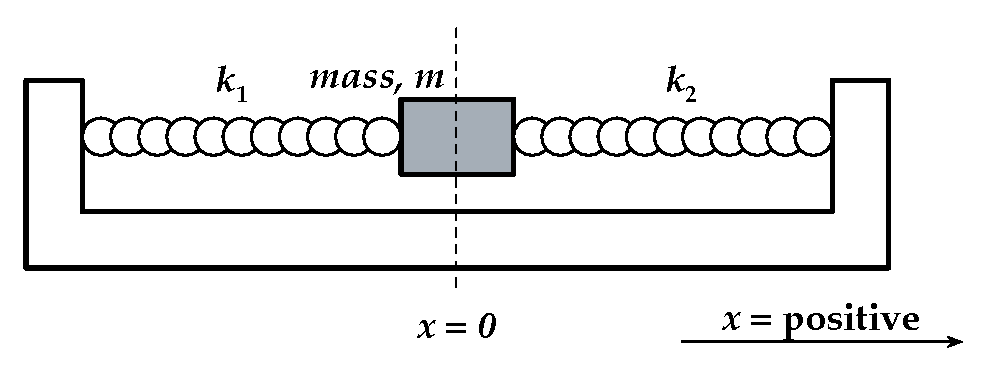
\includegraphics[width=5.5in]{Experiment07Figures/Figure01.pdf}
  \end{center}
  \caption{System sketch for Harmonic Motion experiment.}
  \label{M09Fig01}  % the \label command comes AFTER the caption
\end{figure}

The springs each apply a force according to Hooke's Law as follows
\begin{eqnarray*}
  F_1 & = & -k_1\, x - F_0\\
  F_2 & = & -k_2\, x + F_0.
\end{eqnarray*}
When $x = 0$, each spring pulls an equal and opposite amount $F_0$ resulting in a net force of $F = F_1 + F_2 = 0$ at the center equilibrium position.

When the mass is displaced to some point $x$, the net force $F(x)$ is given by
\[
F(x) = F_1(x) + F_2(x) = -(k_1 + k_2) x.
\]
These two springs acting together in this manner produce a force $F(x) = -k_{eff} x$, where $k_{eff} = k_1 + k_2$, or we can say that the force on the mass acts as if one spring was tied to it with an effective spring constant $k_{eff}$.

If we displace the mass to some position $x = A$ and release it at time $t = 0$, we can determine how the mass will move as a function of time under the influence of the restoring force $F(x)$.  Using Newton's Second Law and the definition of the acceleration $a$, we can write
\begin{equation}
  \label{eq:M09fx}
  F(x) = m\, a = m \frac{{\rm d}^{2}x}{{\rm d} t^{2}} = -k x.
\end{equation}
In order to find a solution to this equation, we need to find a function $x(t)$ whose second derivative is the same as the function itself, give or take a constant or two.  One such function $x(t)$ is
\begin{equation}
  \label{eq:M09xt}
  x(t) = A \cos\left(\omega t \right).
\end{equation}
where $A$ and $\omega$ are constants.  In order to evaluate the constants we observe what the function $x(t)$ must be at known points.  One such point is $t = 0$ where $x = A$, that is the release point of the displaced mass.  If we substitute the function $x(t)$ into Eqn.~\ref{eq:M09fx}, we will find that it satisfies the equation if
\begin{equation}
  \label{eq:M09omega}
  \omega = \sqrt{\frac{k}{m}}.
\end{equation}

The quantity $\omega$ is called the angular frequency.  From Eqn.~\ref{eq:M09xt}, we see that the position of the mass oscillates between the points $+A$ and $-A$ as the cosine function oscillates between $+1$ and $-1$ as a function of time.  The cosine makes one complete oscillation from $+1$ to $-1$ to $+1$ when the quantity $\omega t$ goes through $2\pi$ radians.  The elapsed time for this one complete oscillation is $T$, the period.  Thus $\omega T = 2 \pi$, or
\[
\omega = \frac{2\pi}{T}.
\]

If the period is the time it takes the mass to make one complete cycle, the frequency will be $f = (1/T)$ or $\omega = 2\pi f$.  Using Eqn.~\ref{eq:M09omega} we can write the period as
\begin{equation}
  \label{eq:M09period}
  T = 2 \pi \sqrt{\frac{m}{k}}.
\end{equation}
Note that the period of oscillation is independent of the amplitude $A$ of the oscillation for this case where there are no energy loss mechanisms.

When the system is started, the mass was displaced a distance $A$ and then released.  When the system is displaced that distance $A$, a certain energy is given to the system in the form of potential energy stored in the springs in the amount of $U=(1/2) k A^{2}$.  Thereafter, this initial energy is the total mechanical energy of the system, and without any energy loss mechanisms, the total energy remains constant.  Thus, as the mass moves, it exchanges potential and kinetic energy.  If no energy is lost, the mass will always oscillate between the same amplitude $+A$ and $-A$.  It will also have the same maximum kinetic energy which occurs at the $x = 0$, or equilibrium position.  You can see from Eqn.~\ref{eq:M09xt} and its derivatives, that the displacement, velocity, and acceleration of the mass are related as:
\begin{eqnarray*}
  x(t) &=&  A          \cos(\omega t),\\
  v(t) &=& -A \omega   \sin(\omega t),\\
  a(t) &=& -A \omega^2 \cos(\omega t).
\end{eqnarray*}
The maximum values of $v(t)$ and $a(t)$ are dependent on the amplitude $A$.  Assume now that there is some energy loss mechanism present as the mass oscillates, e.g.\ some friction on the surface on which the mass is sliding or some air drag on the mass.  If energy is lost to such a nonconservative force, then the total energy of the system will decrease.  As the total energy decreases, the amplitude, along with the maximum velocity and acceleration will also decrease.  Since neither the period nor the frequency of oscillation are functions of the amplitude, they should remain constant.  This kind of motion is called damped harmonic motion.

The opposite effect is also true.  If a little bit of energy is added during each cycle, then the total energy of the system will increase and be manifested by an increase in amplitude and still no change in period.

In the laboratory, we will measure the spring constants of two almost identical springs by applying a known force and measuring the stretching (the displacement) of each of the springs.  These two springs will then be configured with a mass on a frictionless surface (a glider on an airtrack) as illustrated in Fig.~\ref{M09Fig01}.  We will set the mass in motion by releasing it from a displacement point and measuring the period of oscillation.  This measured period will be compared with the calculated value obtained from Eqn.~\ref{eq:M09period}.

The independence of the period on amplitude will be examined by measuring the period for the mass started with various amplitudes.  We will also observe the behavior of the motion of the oscillating mass in a case where the energy loss mechanism will be dramatically increased by placing a sail on the glider to increase the air drag.


\pagebreak

\section{Experimental Procedure}

Before assembling the glider and springs on the airtrack, we will determine the spring constants of the two springs.  These very light springs are capable of stretching 20 times their rest length.  Please be very careful not to damage them through careless handling or overstretching.

\begin{figure}
  \centering
  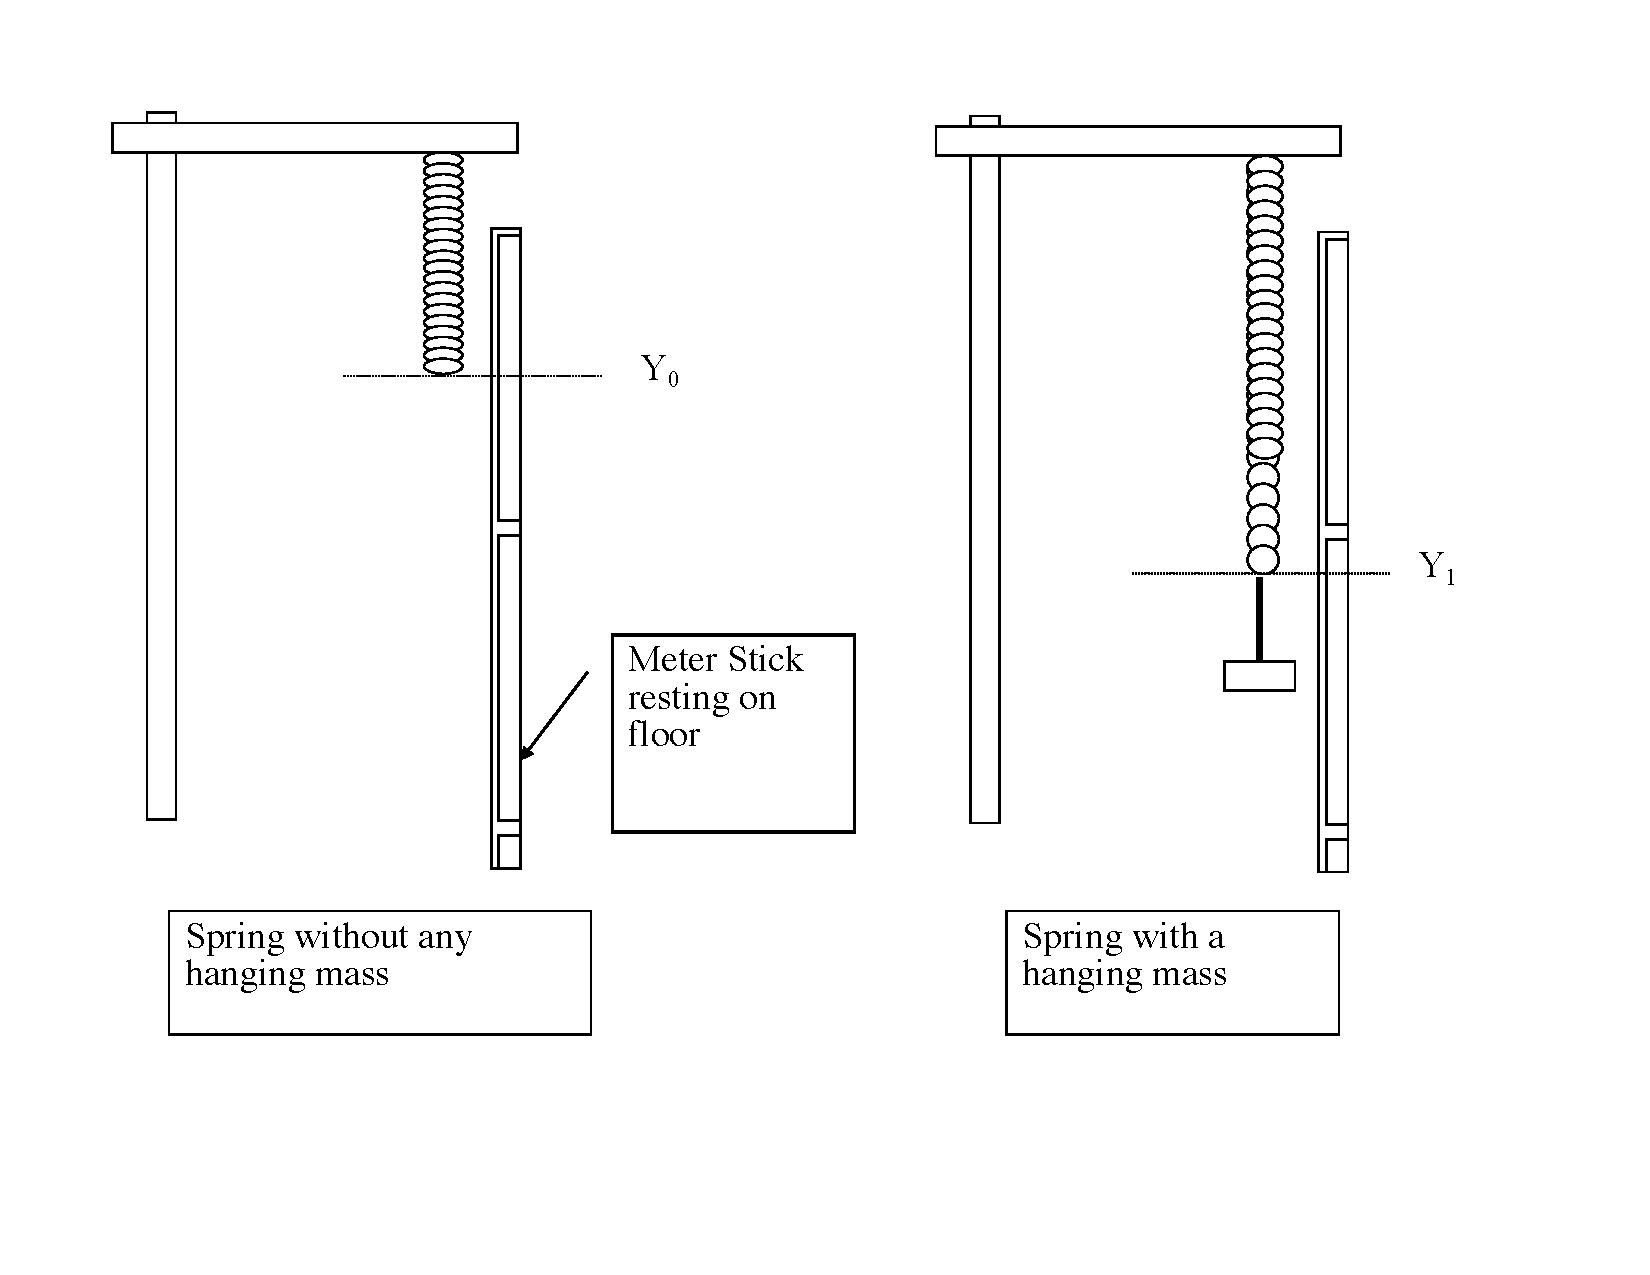
\includegraphics[width=6.0in]{Experiment07Figures/Figure02.pdf}
  \caption{Experimental Method to measure $\Delta y$ for a spring in Experiment M-\ref{lab:M9}}
  \label{M09Fig02}
\end{figure}

\begin{itemize}
\item For each spring perform the following steps to determine its average spring constant $k_{\text{spring }n}$.  Refer to Fig.~\ref{M09Fig02}.
  \begin{enumerate}
  \item Orient the 2-meter stick with the zero end at the top. It is only the change in $y$ with force that matters in this measurement. 
  \item Attach one end of the spring to the ring stand and allow the spring to hang free with no mass hanging. Record $y_0$.
  %\item Carefully hang a 50~\gram\ weight holder on the end of the spring and record $y_1$. Take the measurements with the spring and any weights hanging stationary.
  \item Carefully hang enough mass on a weight holder on the end of the spring until it extends a total displacement of $\sim 0.95 \meter$ from $y_0$ and record the exact distance $y_1$ and mass used as $m_1$ (don't forget the hanger is 50 grams itself). Take the measurements with the spring and any weights hanging stationary.
    %  \item Displace the 50~\gram\ weight holder 2.0~\centi\metre\ release it. Measure the time for 20 oscillations and divide by 20 to obtain the period of the spring with the hanging 50 gram weight holder.
  %\item Add an additional 20~\gram\ to the weight holder and repeat steps 1--3.
  \item Add a additional mass to the weight holder on the end of the spring until it extends a total displacement of $\sim 1.55 \meter$ from $y_0$ and record the exact distance $y_2$ and mass used as $m_2$ (don't forget the hanger is 50 grams itself). Take the measurements with the spring and any weights hanging stationary.
    \item Calculate and record the two values of $k$ for the current spring.  The first is $k_{1\text{,spring1}}=m_1 \,g/(y_1 - y_0)$.  The second is $k_{2\text{,spring1}}=m_2 \,g/(y_2 - y_0)$.
    \item Repeat the above steps for the second spring to find $k_{1\text{,spring2}}$ and $k_{2\text{,spring2}}$.
    %  \item Average the values of $k$ for the spring and record $k$ for that spring and the standard deviation. See Eqn.~\ref{eq:errorSigmaX}.
    %  \item Average the period for that spring and calculate the standard deviation.
  \end{enumerate}
  \item Calculate the average values for $k_{\text{spring1}}$ and $k_{\text{spring2}}$ and then determine the effective spring constant $k_{eff} = k_{\text{spring1}} + k_{\text{spring2}}$ that will be acting on the glider.
\item Turn on the air supply to the airtrack and allow it to flow for several minutes.
\item Measure the mass of the larger glider and place it on the track.
\item \textbf{CASE 1:} Use the scale on the track and a corner of a glider to determine various displacements along the track.
  \begin{enumerate}
  \item Assemble the larger glider on the track and attach the springs to the glider and the ends of the track as in Fig.~\ref{M09Fig01}.  Again please be careful not to overstretch the springs or allow them to snap back.
  \item To determine the period of oscillation of the mass, displace the mass 10~\centi\metre\ from its equilibrium position and release it. When the mass returns to its starting point, start the stopwatch at the zero velocity point.  Allow the mass to oscillate through 10 complete cycles and stop the stopwatch at the zero velocity point at the end of the tenth cycle. That will be essentially the starting point.  Record the time for the ten cycles and divide by 10 to obtain the period.
  \item Using the same cart, find the period for starting amplitudes of 15, 20, 25, and 30~\centi\metre.
  \item Calculate the expected period from Eqn.~\ref{eq:M09period} and compare it with each of the measured values for the different starting amplitudes.
  \end{enumerate} 
\item \textbf{CASE 2 \& 3:} Measure the mass of the small glider with and without the sail-holder and sail. Reassemble the system with the smaller glider without the sail assembly on the track.
  \begin{enumerate}
  \item Using the same measuring technique as used with the larger glider, determine the period for a starting amplitude of 10~\centi\metre.  Record the time for ten cycles and divide by 10 to obtain the period.
  \item Using the same cart, find the period for starting amplitudes of 15, 20, 25, and 30~\centi\metre.
  \item Calculate the expected period from Eqn.~\ref{eq:M09period} and compare it with each of the measured values for the different starting amplitudes.
  \item Place the paper sail assembly on the glider.
  \item Use a starting amplitude of 25~\centi\metre\ from the equilibrium position.  Record both the equilibrium position and your starting point; determine and record the amplitude (should be 25 cm).  Each of the following steps will be started from this same amplitude point.
    %\item Pick a convenient amplitude point approximately 25~\centi\metre\ (but NOT greater than 30~\centi\metre!) from the equilibrium position.  Record both the equilibrium position and your starting point; determine and record the amplitude.  Each of the following steps will be started from this same amplitude point.
    \begin{enumerate}%[label=(\Alph*)]
    \item Displace the glider with its sail to the starting point and release it.  At the end of the fifth cycle, capture the glider by gently pressing your finger on the edge of the glider as gets to its maximum amplitude point, i.e.\ $v = 0$.  Record the amplitude.  Be sure to use the same point on the glider that you used to determine the equilibrium point and the 25~\centi\metre\ starting point.  Measure the total time for the cycles and divide by the number of cycles measured to obtain the average period.  Compare this with the expected period from Eqn.~\ref{eq:M09period}.  (Use the total mass of the glider and sail assembly as the mass.)
    \item Repeat step (A) five more times, each time starting the glider from the 25~\centi\metre\ point and allowing it to cycle five more cycles than the previous measurement. \textbf{Only 1 trial needed per number of cycles.}
    \end{enumerate}
  \end{enumerate}
\end{itemize}


\section{Data Analysis}
Create tables for each of the two springs to measure the spring constant by measuring the extension of the spring at two different displacements from $y_0$, $\sim 0.95 \meter$ and $\sim 1.55 \meter$.
\begin{itemize}
\item Create a table for each spring with a row for each displacement trial including:
  \begin{itemize}
  \item The height $y_0$ of the bottom of the loop on the spring (no mass)
  \item the applied mass (including hanger)
  \item the gravitational force due to the mass
  \item the height $y_n$ of the bottom of the loop on the spring with the mass
  \item the displacement $y_n-y_0$ due to the mass
  \item the spring constant
%  \item the period of a small oscillation of the mass.
  \end{itemize}
%\itemFor each spring, compare the period measured with the 50 and 70~\gram\ masses hanging on the spring to the calculated periods using the spring constant for the spring.
\end{itemize}

Now that the springs are characterized, create tables for the measurement of oscillations of gliders on the air track.
\begin{itemize}
\item Create separate tables for the large and small gliders including the common data of the glider masses and their expected periods. Create a row for each trial. There are 15 trials for each glider --- from three repetitions (trials) for each of the five initial amplitudes (cases). \textbf{NOTE: Have each group member measure at the same time to be able to save time while still getting 3 trials per amplitude (if there are groups of two people, have someone hold two stopwatches to get the 3 trials).}
  \begin{itemize}
  \item the starting amplitude (displacement from equilibrium) in meters (0.10, 0.15, 0.2, 0.25, and 0.3~\meter)
  \item the time for ten cycles
  \item determined period
  \end{itemize}
\item For each glider calculate the mean and standard deviation of the period.
\end{itemize}

The third experiment in this lab focuses on measuring the damped oscillation of the small glider with a sail.
\begin{itemize}
\item Record the mass of the small glider with the sail assembly, calculate the expected period and observe the resting location of the glider $A_0$. Calculate and record the starting point $A_0 + 0.250\,\meter$. \textbf{Reminder, only 1 trial needed per number of cycles.}
\item Create a row for each of the 6 number-of-cycles trials including:
  \begin{itemize}
  \item the number of cycles
  \item the ending point
  \item the ending amplitude (ending point minus equilibrium point)
  \item the total time
  \item the average period
  \end{itemize}


\item Plotting:
\begin{itemize}
    \item For all three cases produce a graph of the period $T$ ($y$-axis) vs. the amplitude $A$ ($x$-axis).
    \item For the third case produce a graph of the amplitude $A$ ($y$-axis) vs. the number of cycles ($x$-axis). Use the starting amplitude $A_0$ as the value for zero cycles.
    \item Draw a line-of-best-fit through the data points for each plot.
\end{itemize}

\end{itemize}



\pagebreak


\section{Post-Lab Submission --- Interpretation of Results}

\begin{itemize}
\item Make sure to submit your finalized data table (Excel sheet)
\item For all three cases, do the the measured periods of the glider agree with the expected value?
\item What are the uncertainties? How would those uncertainties affect the measured period?

\item Comment (qualitatively) on the behavior of the curves from each plot. Do the trends make sense?
\item From the damped-oscillator plot, what do you expect amplitude of the glider to be after 50 cycles?

%\item In a perfect system, would the glider ever truly reach an amplitude of zero?

%\item For each spring, compare the period measured with the 50 gm and 70 gm masses hanging on the spring to the calculated periods using the spring constant for the spring,  $k_1$ or $k_2$ and Eqn.~\ref{eq:M09period}. Explain why the measured period is different from the calculated period [Hint: What mass is moving?].

\item Does the amplitude affect the period? Why or why not?
\item How does the period depend on the mass of the glider? Is this expected?
\item How does an increased air drag affect the result for the period?
\subitem How does the amplitude depend on the number of cycles (relate this to energy conservation)?

\item What are possible systematic errors for today's experiments?


\end{itemize}

